\documentclass[tikz,border=5pt]{standalone}
\usepackage{tikz}
\usetikzlibrary{arrows.meta, positioning, fit, backgrounds, decorations.pathreplacing, calc}

\begin{document}
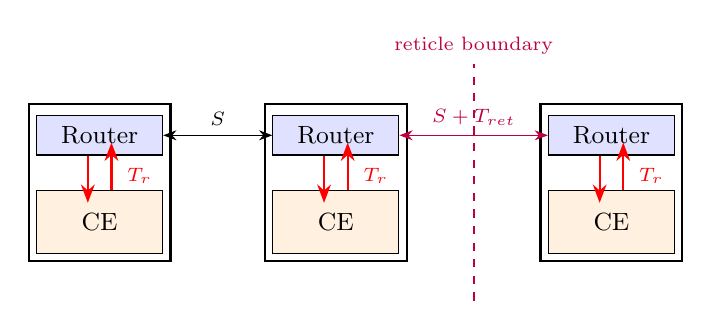
\begin{tikzpicture}[
        font=\small,
        pe/.style={draw, thick, minimum width=1.8cm, minimum height=2cm},
        router/.style={draw, fill=blue!12, minimum width=1.6cm, minimum height=0.5cm},
        ce/.style={draw, fill=orange!12, minimum width=1.6cm, minimum height=0.8cm},
        linklabel/.style={font=\scriptsize, align=center},
        >=Stealth
    ]


    % ---- PE 2 ----
    \node[pe] (pe2) at (3,0) {};
    \node[router] (r2) at (3,0.6) {Router};
    \node[ce] (c2) at (3,-0.5) {CE};

    % ---- PE 3 ----
    \node[pe] (pe3) at (6,0) {};
    \node[router] (r3) at (6,0.6) {Router};
    \node[ce] (c3) at (6,-0.5) {CE};

    % ---- PE 4 (across reticle boundary) ----
    \node[pe] (pe4) at (9.5,0) {};
    \node[router] (r4) at (9.5,0.6) {Router};
    \node[ce] (c4) at (9.5,-0.5) {CE};

    % ---- router-to-router latency S (PE2 -> PE3) ----
    \draw[<->] (r2.east) -- node[linklabel, above] {$S$} (r3.west);

    % ---- ramp latency Tr: router -> compute engine (down) and CE -> router (up), shown on PE2 ----
    \draw[->, red, thick] ($(r2.south)+(-0.15,0)$) -- ++(0,-0.6);
    \draw[->, red, thick] ($(c2.north)+(0.15,0)$) -- ++(0,0.6)
    node[linklabel, red, right, xshift=2pt, yshift=-12pt] {$T_r$};



    % ---- ramp latency Tr: router -> compute engine (down) and CE -> router (up), shown on PE2 ----
    \draw[->, red, thick] ($(r3.south)+(-0.15,0)$) -- ++(0,-0.6);
    \draw[->, red, thick] ($(c3.north)+(0.15,0)$) -- ++(0,0.6)
    node[linklabel, red, right, xshift=2pt, yshift=-12pt] {$T_r$};

    % ---- ramp latency Tr: router -> compute engine (down) and CE -> router (up), shown on PE2 ----
    \draw[->, red, thick] ($(r4.south)+(-0.15,0)$) -- ++(0,-0.6);
    \draw[->, red, thick] ($(c4.north)+(0.15,0)$) -- ++(0,0.6)
    node[linklabel, red, right, xshift=2pt, yshift=-12pt] {$T_r$};

    % ---- reticle boundary between PE3 and PE4 ----
    \draw[dashed, thick, purple] ($(pe3.east)!0.5!(pe4.west)$) ++(0,-1.5) -- ++(0,3.0)
    node[above, purple, font=\scriptsize] {reticle boundary};


    % ---- router-to-router latency across reticle: S + Sret ----
    \draw[<->, purple] (r3.east) -- node[linklabel, above] {$S + T_{ret}$} (r4.west);


\end{tikzpicture}
\end{document}
